\documentclass[tikz]{standalone}
\usetikzlibrary{calc,positioning}
\begin{document}
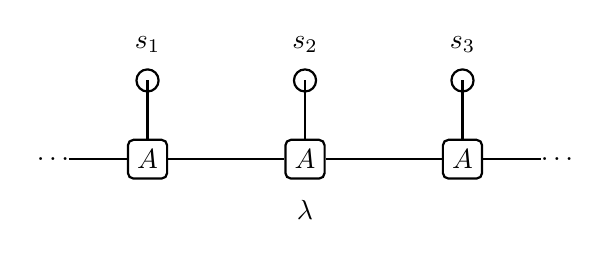
\begin{tikzpicture}[baseline={([yshift=-.5ex]psi.center)},
    tensor/.style={draw,thick,minimum size=14pt,rounded corners=2pt},
    phys/.style={draw,thick,circle,minimum size=8pt,inner sep=1pt}]
  \node[tensor] (A1) at (0,0) {$A$};
  \node[tensor] (A2) at (2,0) {$A$};
  \node[tensor] (A3) at (4,0) {$A$};
  \draw[thick] (-1,0) -- (A1);
  \draw[thick] (A1) -- (A2);
  \draw[thick] (A2) -- (A3);
  \draw[thick] (A3) -- (5,0);
  \foreach \x in {1,2,3} {
    \draw[thick] (A\x) -- ++(0,1) node[phys] (p\x) {};
    \node[above=2pt of p\x] {$s_{\x}$};
  }
  \node at (-1.2,0) {$\dots$};
  \node at (5.2,0) {$\dots$};
  \node[below=4pt of A2] (psi) {$\lambda$};
\end{tikzpicture}
\end{document}
